\documentclass[12pt]{article}

\usepackage{fullpage}
\usepackage{multicol,multirow}
\usepackage{tabularx}
\usepackage{listings}
\usepackage{pgfplots}
\usepackage[utf8]{inputenc}
\usepackage[russian]{babel}
\usepackage[T2A]{fontenc}
\usepackage{pgfplots}
\usepackage{tikz}


\begin{document}

% \newpage
% \begin{center}
% {\bfseries ФЕДЕРАЛЬНОЕ ГОСУДАРСТВЕННОЕ БЮДЖЕТНОЕ ОБРАЗОВАТЕЛЬНОЕ\\
% УЧРЕЖДЕНИЕ ВЫСШЕГО ОБРАЗОВАНИЯ\\
% «МОСКОВСКИЙ АВИАЦИОННЫЙ ИНСТИТУТ\\
% (НАЦИОНАЛЬНЫЙ ИССЛЕДОВАТЕЛЬСКИЙ УНИВЕРСИТЕТ)»}
% \vspace{1cm}

% Журнал лабораторных работ
% \vspace{6em}

% \vspace{\fill}

% \begin{center}
% Москва 2024
% \newpage
% \end{center}

\section*{Лабораторная работа №5\, по курсу компьютерной графики}

\textbf{Тема:} Трассировка лучей (Ray Tracing)\\
\\
\textbf{Задача:} В этой лабораторной работе вы научитесь работать с техникой трассировки лучей для
создания реалистичной 3D-графики. Вы реализуете алгоритм Ray Tracing, который позволяет
рассчитывать физически корректные отражения, преломления, тени и свет в сцене.
Лабораторная работа подводит к пониманию основ рендеринга, работающего с лучами
света, а также к созданию реалистичных сцен.\\
\textbf{Вариант:} 2. \\
Постройте сцену с одной сферой и одной плоскостью (пол).\\
Реализуйте направленный источник света, который отбрасывает тени на объект.\\
Реализуйте мягкие тени (soft shadows) с помощью распределенной трассировки лучей.\\
Дополнительно: Реализуйте возможность изменения размера источника света, чтобы
контролировать степень мягкости теней.\\

\subsection*{1 Решение}
В лабораторной работе реализован алгоритм трассировки лучей на C++. 
Создана сцена с одной сферой и плоскостью, добавлен направленный источник света. 
Для получения мягких теней использована распределённая трассировка лучей с учётом размера источника света. 
Реализован расчёт диффузного освещения, тени и цвета объектов. Результат рендеринга сохраняется в формате PPM.

\begin{figure}[h]

\centering
        
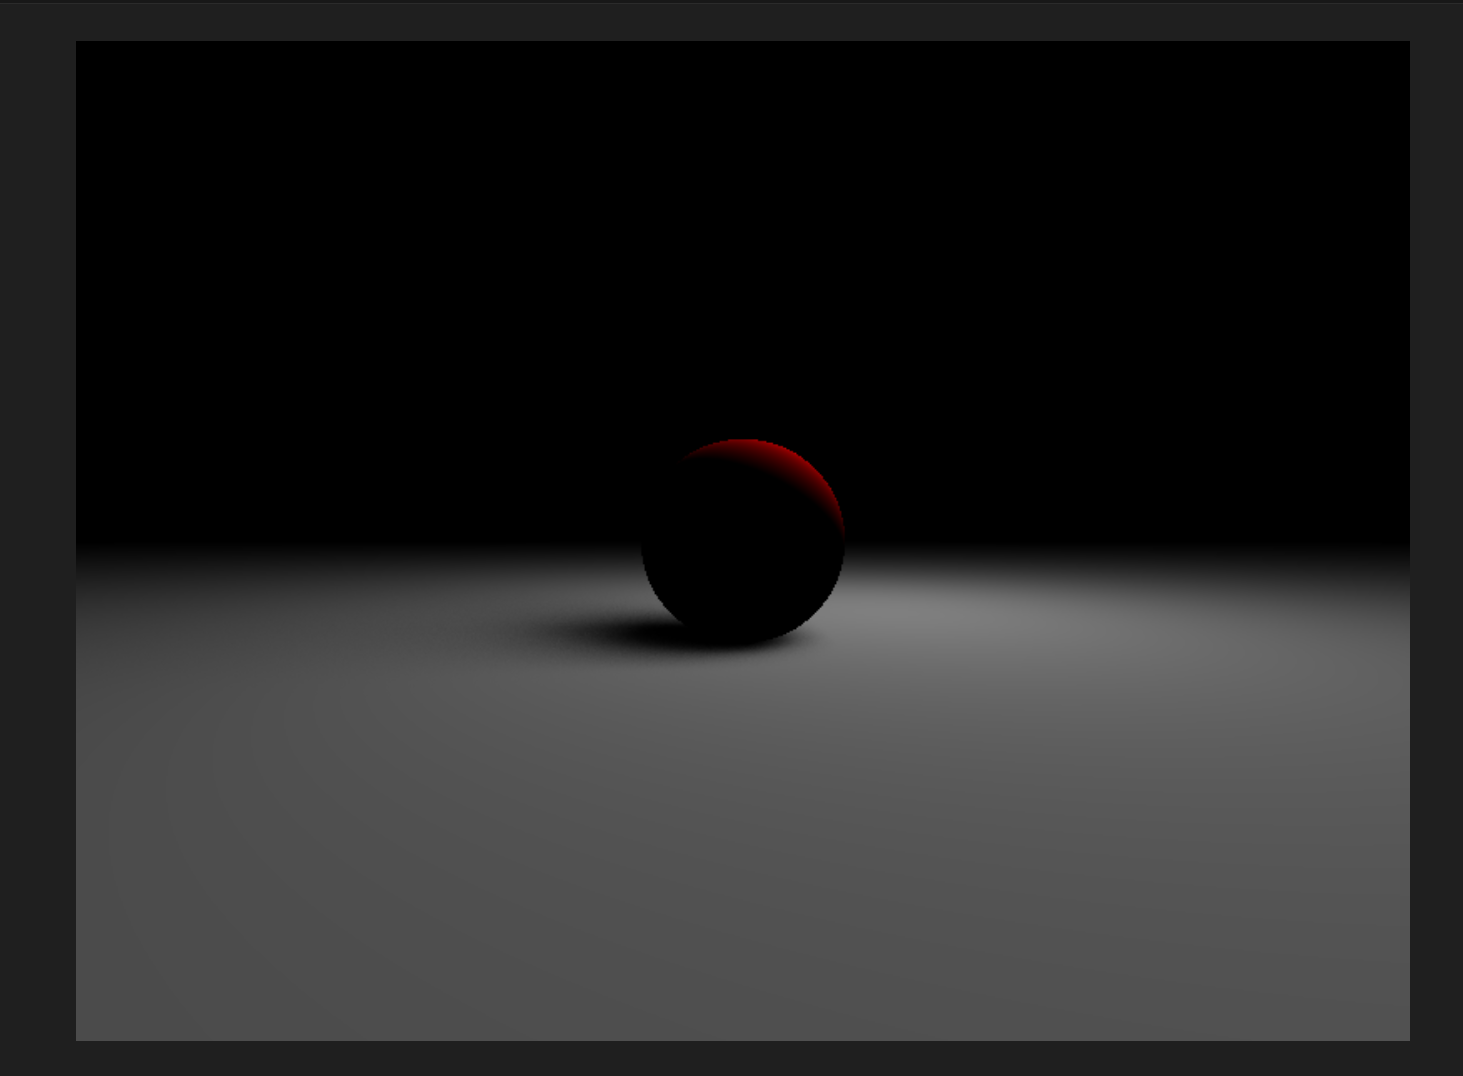
\includegraphics[width=0.8\linewidth]{image.png}
        
\caption{Пример работы программы}
        
\label{fig:mpr}
        
\end{figure}

\subsection*{2 Вывод}
В ходе работы изучены принципы трассировки лучей, реализована генерация мягких теней и управление размытостью через размер источника света. 
Итоговая программа позволяет создавать фотореалистичные изображения.
\end{document}
